\documentclass[12pt]{article}
%\usepackage[margin=1in]{geometry}
\usepackage[left=2.5cm, right=2.5cm, top=2cm]{geometry}
\usepackage{amsmath, amsthm, amssymb, amsfonts}
\usepackage{scrextend}
\usepackage{graphicx}
\usepackage{multicol}
\usepackage{hyperref}


% Set up stuff to handle Python code nicely.
\usepackage{listings}
\usepackage{color}

\definecolor{codegreen}{rgb}{0,0.6,0}
\definecolor{codegray}{rgb}{0.5,0.5,0.5}
\definecolor{codepurple}{rgb}{0.58,0,0.82}
\definecolor{backcolour}{rgb}{0.95,0.95,0.92}

\lstdefinestyle{mystyle}{
    backgroundcolor=\color{backcolour},
    commentstyle=\color{codegreen},
    keywordstyle=\color{magenta},
    numberstyle=\tiny\color{codegray},
    stringstyle=\color{codepurple},
    basicstyle=\footnotesize,
    breakatwhitespace=false,
    breaklines=true,
    captionpos=b,
    keepspaces=true,
    numbers=left,
    numbersep=5pt,
    showspaces=false,
    showstringspaces=false,
    showtabs=false,
    tabsize=2
}

\lstset{style=mystyle}

\setlength{\columnsep}{0.3in}

\newcommand{\N}{\mathbb{N}}
\newcommand{\Z}{\mathbb{Z}}
\newcommand\textlcsc[1]{\textsc{\MakeLowercase{#1}}}
\newcommand{\angstrom}{\textup{\AA}}

\newenvironment{problem}[2][Problem]{\begin{trivlist}
\item[\hskip \labelsep {\bfseries #1}\hskip \labelsep {\bfseries #2.}]}{\end{trivlist}}
%If you want to title your bold things something different just make another thing exactly like this but replace "problem" with the name of the thing you want, like theorem or lemma or whatever

\newenvironment{answer}[2][Answer]{\begin{trivlist}
\item[\hskip \labelsep {\bfseries #1}\hskip \labelsep {\bfseries #2.}]}{\end{trivlist}}


% Enable one-column figures in multicol.
\newenvironment{Figure}
  {\par\medskip\noindent\minipage{\linewidth}}
  {\endminipage\par\medskip}


\begin{document}

%\renewcommand{\qedsymbol}{\filledbox}
%Good resources for looking up how to do stuff:
%Binary operators: http://www.access2science.com/latex/Binary.html
%General help: http://en.wikibooks.org/wiki/LaTeX/Mathematics
%Or just google stuff

% \title{AST 221: Problem Set 1}
% \author{Jonas Powell}
% \maketitle


% make title bold and 14 pt font (Latex default is non-bold, 11 pt)
\title{\Large \textbf{Galactic Astronomy: Problem Set 3}}

\author{{\rm Jonas Powell, \textit{Wesleyan University}}}


\maketitle


\begin{addmargin}[4em]{4em}
\noindent {\bf Due: Thursday, Feb. 28 by midnight.} Late papers are not accepted. If you cannot complete the assignment, hand in what you have completed before the deadline. Consider the deadline to be like the boarding time for an airplane, or the deadline for a grant submission to NASA or NSF. If you miss the deadline, you do not get on the airplane, no matter how good your excuse is. If you miss an NSF or NASA deadline, you do not get the grant, no matter how good your project is. The best advice is ... finish early. You can submit multiple times, right up to the deadline. Whatever your latest submission is, when the deadline occurs, is what will be graded.
\bigskip \bigskip
\end{addmargin}


% Begin two-column layout
% if using this, change margins (line 3) to like 1cm-ish
%\begin{multicols*}{2}


\begin{problem}{1}
  There is an error in the book on page 108? What correction is required?
\end{problem}

\begin{answer}{1}
  On page 108, the author claims that, in the high-T regime, Planck's Law reduces to $B_\nu(T) = (2kT \nu^2)/(h c^2)$. This is not the case; the author has left an extra factor of $h$ in the denominator. Instead, the Rayleigh-Jeans law says that $B_\nu(T) = 2kT \nu^2 c^{-2}$.
\end{answer}



\begin{problem}{2} Become familiar enough with stellar spectra that you can easily classify, at a glance, almost any spectrum into one of the main classes (OBAFGKM) to within plus or minus 1 class. Note that I am not talking about subclasses here, i.e telling a G2 star from a G3 star, which is difficult. I am talking about telling a G star from an A star or an M star. As an illustration of your prowess, how would you classify each of the stars shown below.

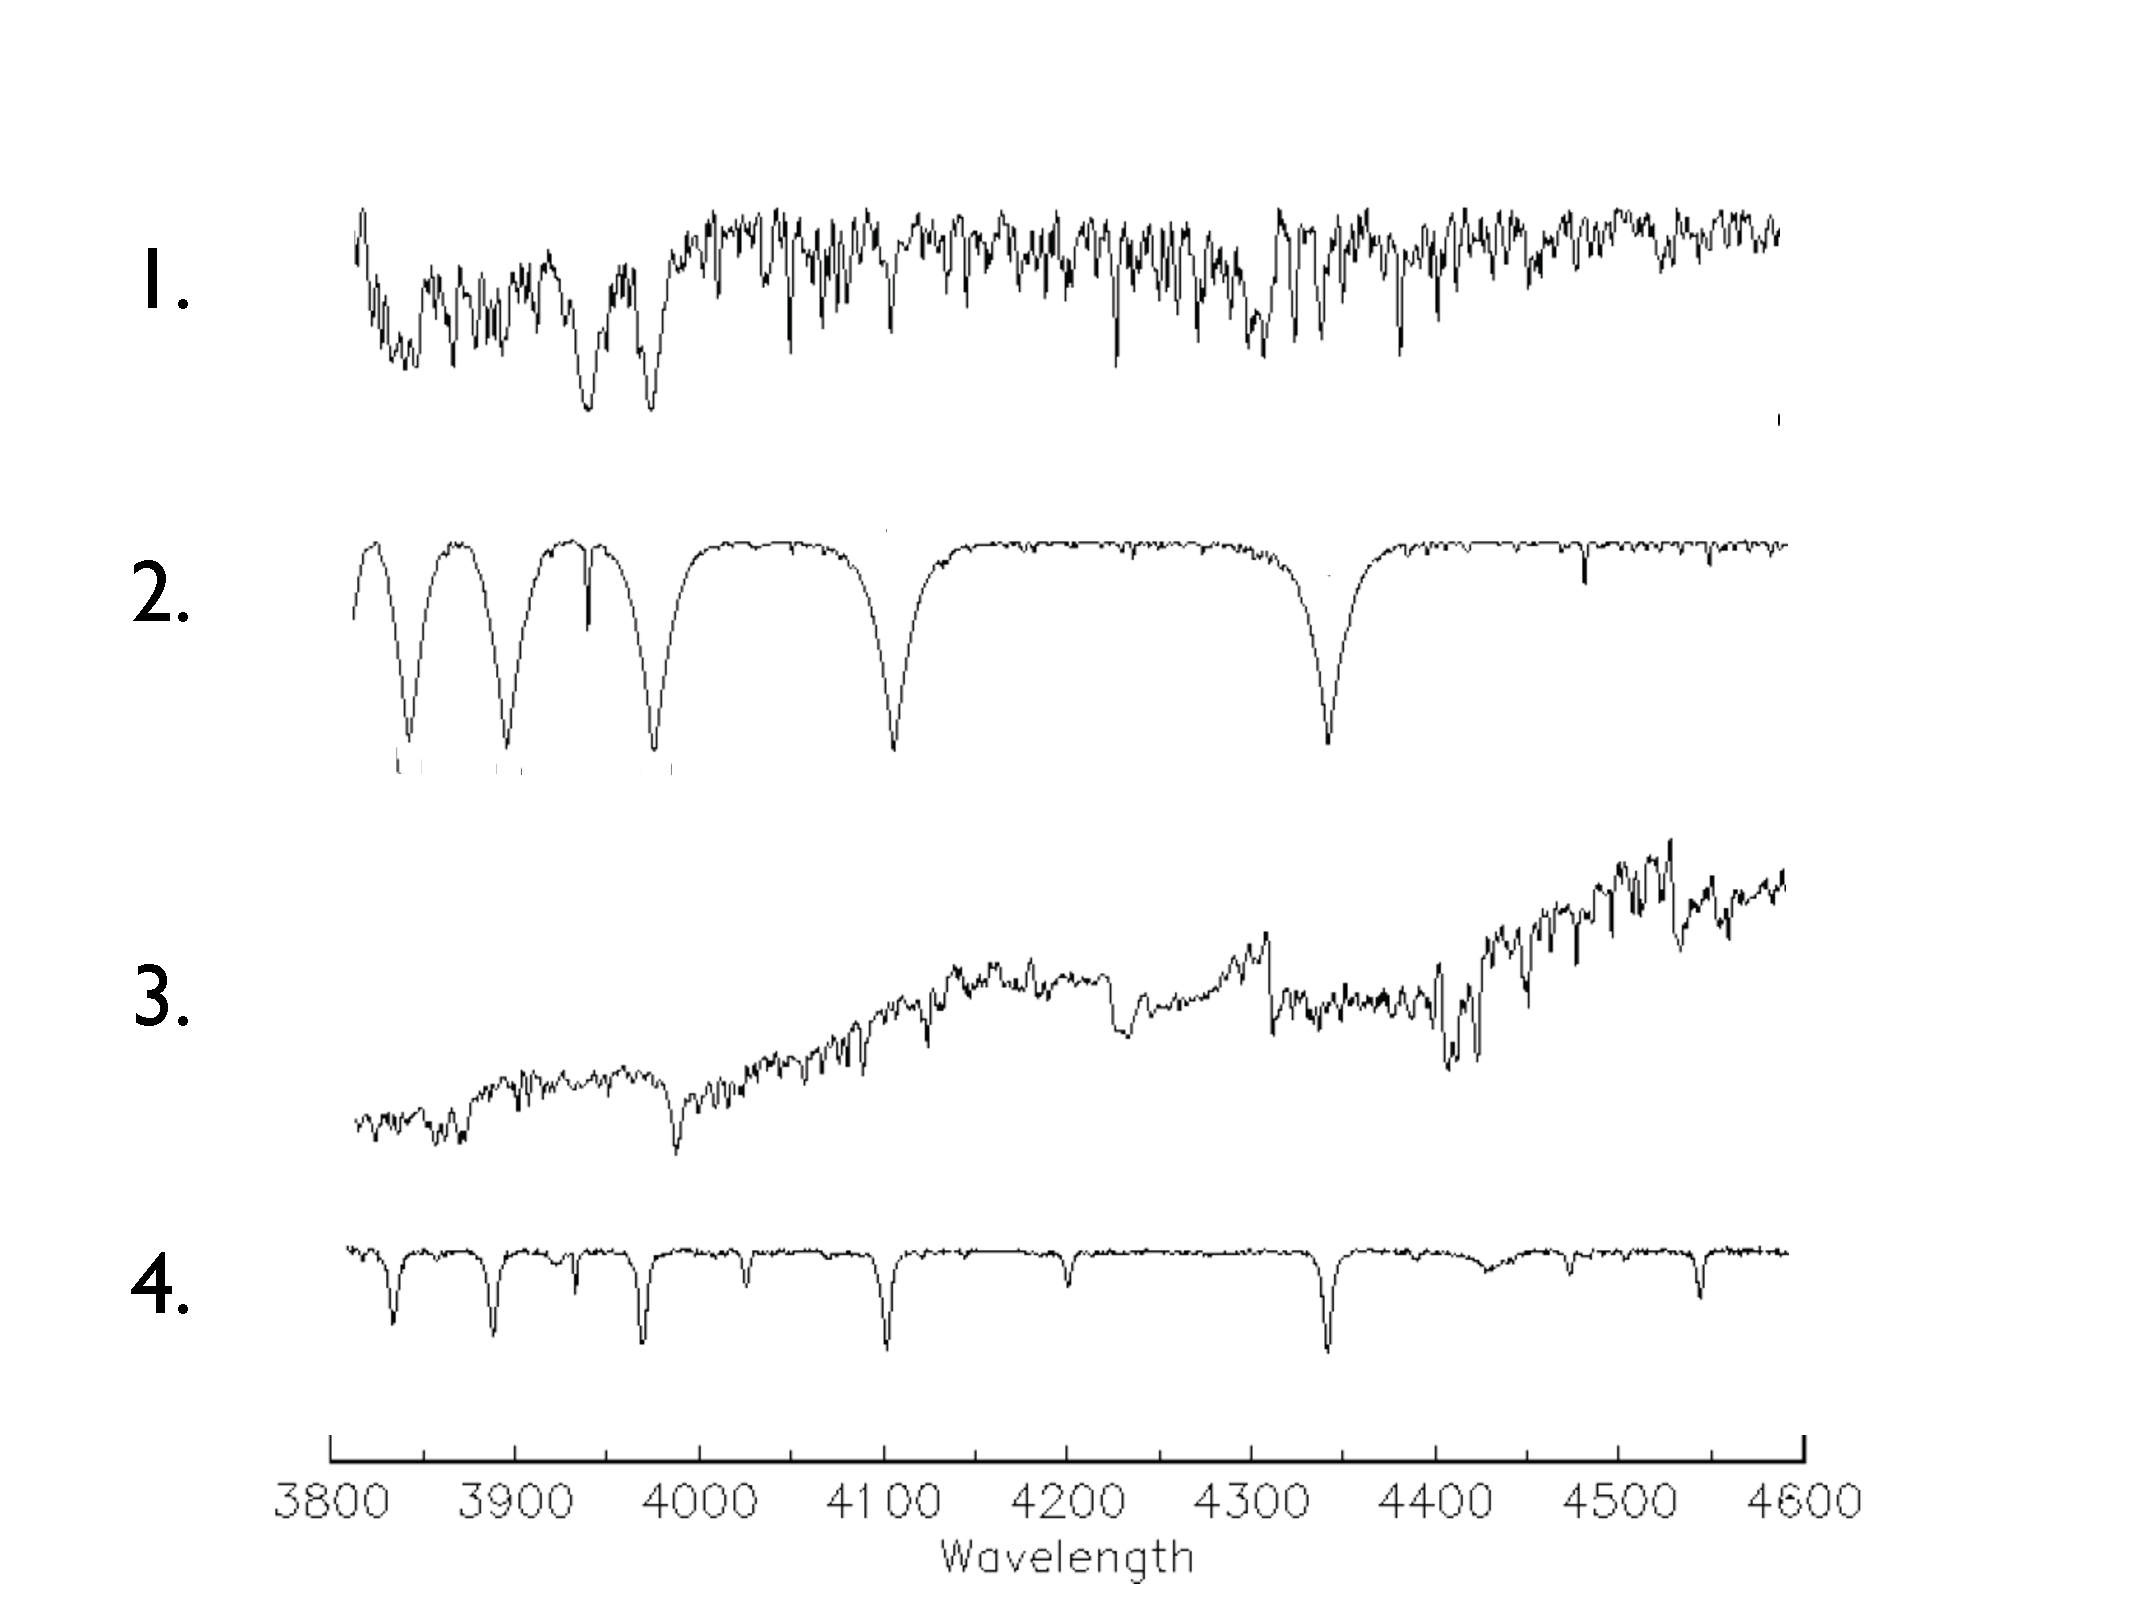
\includegraphics [scale=0.3] {UnknownSpectra.pdf}
\end{problem}

\begin{answer}{2}
  These are my classifications:
  \begin{itemize}
    \item Spectrum 1 is a K-star. We can tell this by its two distinctive absorption lines between 3900 and 4000\angstrom, which are characteristic of K stars.
    \item Spectrum 2 is likely an A-star (or maybe a B), because of its generally clean, featureless spectrum save for large, clear lines.
    \item Spectrum 3 is an M-star. We can tell this because it does not have the major lines that Spectrum 1 had, but rather just a generally choppy surface that indicates an M-star.
    \item Spectrum 4 is an O-star. We know this because, like Spectrum 2, it is generally quite clean and free of minor features, but the significant lines that it does have are shallower than those of Spectrum 2, indicating that it is likely an O.
  \end{itemize}}
\end{answer}



\begin{problem}{3}
  Make an HR diagram that compares a sample of the nearest stars (100 or so would do) with a sample of the brightest stars (chosen by apparent magnitude). The Sun, of course, will be in both data sets, since it is the nearest and the brightest. Plot everything on the same diagram and use different symbols and/or colors to differentiate between the nearest and the brightest.

  There are a variety of catalogs you could use for this, including Gaia, Hipparcos, Gliese, Yale, etc. You may choose where to get your data and exactly what quantities you wish to plot. For example, luminosities could be in terms of M$_V$, M$_{bol}$, L/L$_\odot$, etc. and effective temperatures could be in terms of B-V, some other color index, T$_e$, etc. These are up to you! Make a great looking plot and then describe it and what it tells you about the stellar population in the Galaxy (and other galaxies, as it turns out).
\end{problem}

\begin{answer}{3}

  % \begin{figure}
  %   \begin{minipage}[c]{0.58\textwidth}
  %     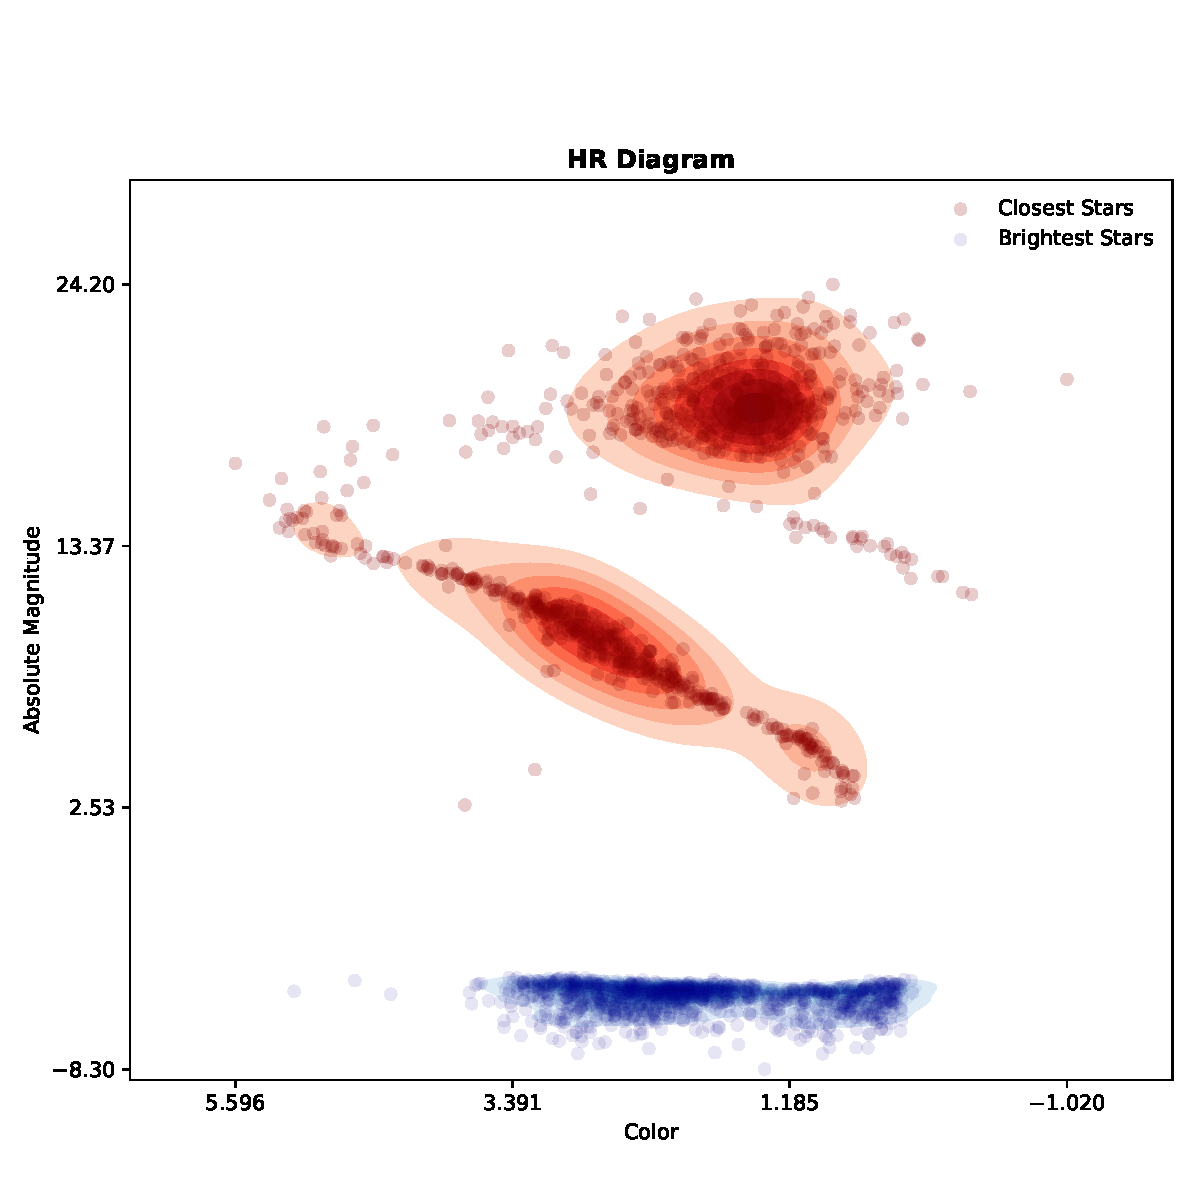
\includegraphics[width=\textwidth]{HR_diagram.pdf}
  %   \end{minipage}\hfill
  %   \begin{minipage}[c]{0.4\textwidth}
  %     \caption{a caption blah blah blah} \label{fig:HRD}
  %   \end{minipage}
  % \end{figure}


\begin{figure}[htp]
  \hspace*{\fill}%
  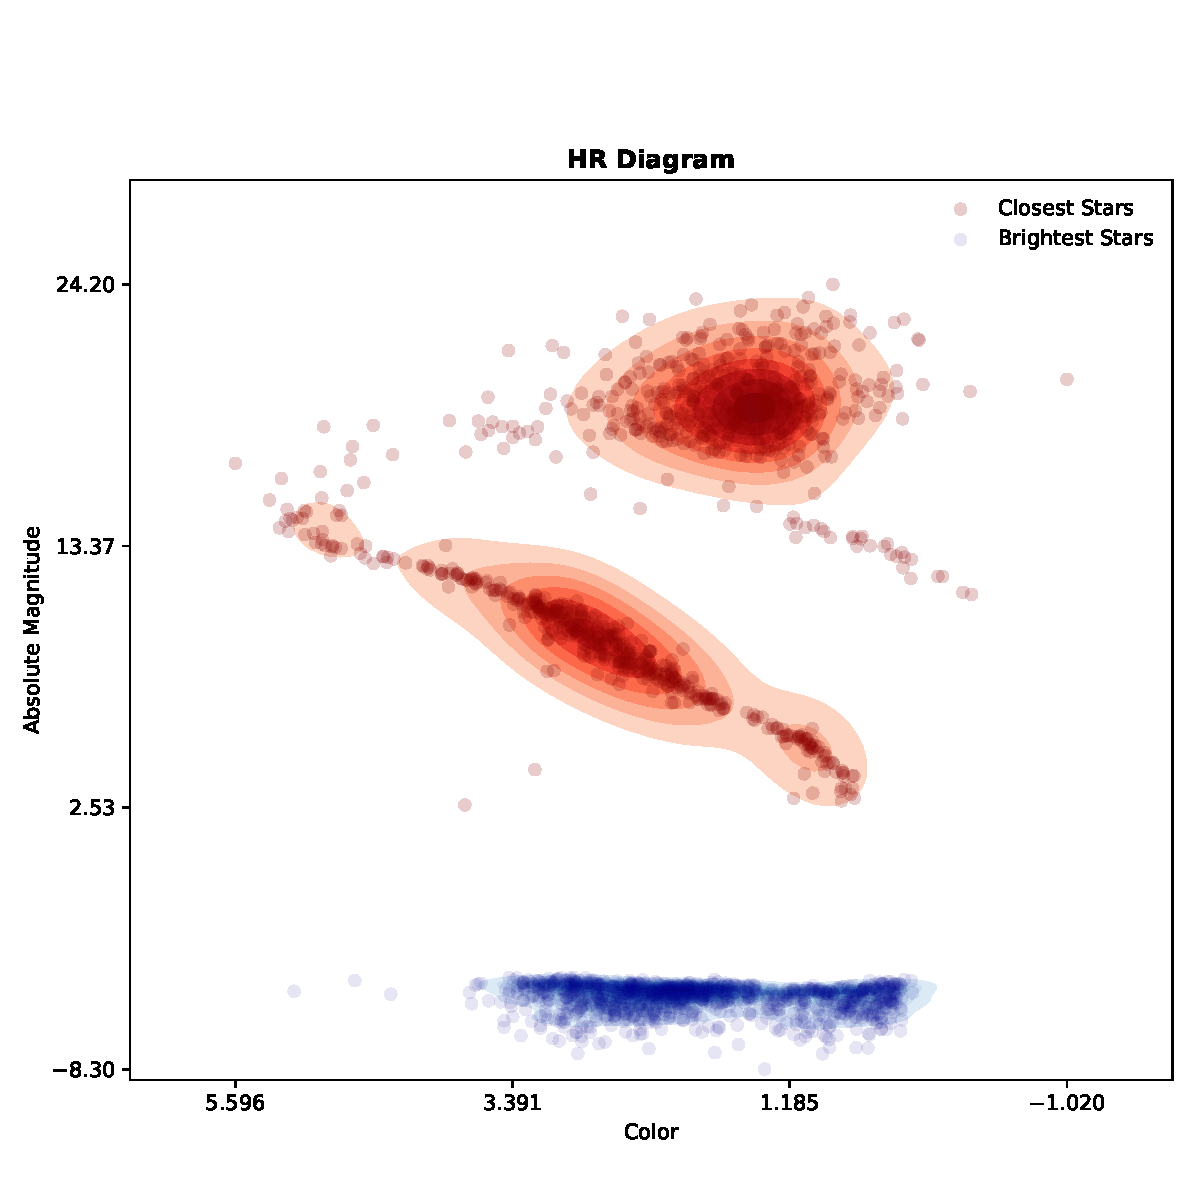
\includegraphics[width=\linewidth]{HR_diagram.pdf}\hfill%
  \hspace*{\fill}%
  \caption{The HR Diagram, composed of the nearest thousand stars and the brightest thousand stars.}
  \label{fig:HRD}
\end{figure}


First off: As I look back over this, I'm finding some weirdness in my Gaia query and am seeing that reflected here. However, I think the overarching message is still alright, but if I had more time, this is something I would go back and fix.

Given the enormity of Gaia and the value of large numbers, I chose to select the thousand brightest and thousand nearest stars. This yielded a more filled HR diagram, obviously, but visual inspection showed that it didn't change the qualitative structure of it much.

We immediately may see that the brightness cutoff we implemented, selecting only the top $n$ brightest stars, is working by the fact that all those stars selected by brightness are clustered below some cutoff line on the y-axis. These stars tend to be clustered within a fairly non-extreme color range, from about 0 to 3.4.

The stars closest to us, of course, are much more evenly distributed across the HR diagram. Oddly, it seems like a significant portion of the stars are giants.

\end{answer}



\begin{problem}{4}
  Determine the stellar number density and mass density in the solar neighborhood based on the sample of the 100 or so nearest stars that you used in problem 3. Note that you will need to assign masses to these objects, using a mass-luminosity relationship, which you adopt. Report your results in several different ways, so that you can get a feeling for what they mean. In particular, give the number density in units of stars per pc$^{-3}$, and the mass density in terms of M$_\odot$ pc$^{-3}$, gm cm$^{-3}$, and H-atoms cm$^{-3}$.
\end{problem}

\begin{answer}{4}
  Using the same Gaia data that we used above, we may calculate varies densities in the local Universe. These numbers may be bad, reflecting the same errors I likely made above. Still, I think the logic behind my derivations is reasonable.
%   Stars per Cubic Parsec:  0.07077745884416348
%   Solar Masses per Cubic Parsec:  0.05852295414109303
%   Grams per Cubic Centimeter:  3.983904086158409e-24
%   Hydrogen Atoms per Cubic Centimeter:  2379.871019210518

\bigskip
\centerline{\textbf{Densities}}
\smallskip
\centerline{
  \begin{tabular} {c | l}
  \hline \hline
  N$_{\text{stars}}$ pc$^{-3}$    & 0.071 \\
  M$_\odot$ pc$^{-3}$         & 0.058 \\
  gm cm$^{-3}$                & 3.984 \times 10^{-24} \\
  N$_{H}$ cm$^{-3}$             & 2379.87 \\
  \hline
  \end{tabular}}
\end{answer}
\bigskip \bigskip

How I found these values:
\begin{itemize}
  \item \textsc{N$_{\text{stars}}$ pc$^{-3}$}: We may find a number density by dividing the total number of stars in the sample by a volume. For this volume, I chose to make a cube whose side length was the distance of the most distant star in the sample.
  \item \textsc{M$_\odot$ pc$^{-3}$}: To find mass density, we may simply multiply our number density by the sum of the sample's masses. As instructed, the mass attribute for each source was calculated using the mass/luminosity relationship.
  \item \textsc{gm cm$^{-3}$}: This mass density can be calculated by scaling the above mass density by the relevant conversion factors, i.e. M$_\odot$-to-gm and (pc-to-cm)$^{-3}$.
  \item \textsc{N$_{H}$ cm$^{-3}$}: To find the number density of hydrogen, I began by assuming that all stars were made up purely of hydrogen (i.e. $M_H = M_\text{stars}$). I then turned converted this value from solar masses to grams and then grams to number of hydrogen atoms. I then divided this number, as above, by the cube of the largest distance in the dataset. This yielded a value that was much higher (of order a couple thousand) than what I expected (around 1); not totally sure where this went wrong but I think it's likely just a conversion factor.
\end{answer}




\begin{problem}{5}
  Prove that, if the orbital planes of binaries are oriented randomly with respect to the plane of the sky, then the average value of sin$^3 i$ for the binaries is $\langle \sin ^3 i \rangle$ = 0.59.
\end{problem}

\begin{answer}{5}
We may approach this problem in one of two ways: we may numerically simulate observations or analytically solve it.

The analytical method seems to be the better path. To do so, we begin by recalling the definition of $\langle x \rangle$:
\begin{align*}
  \langle x \rangle = \int x\ P(x) dx
\end{align*}

Since we are looking for the average value of sin$^3 i$, then this equation becomes
\begin{align*}
  \langle\sin^3 i\rangle = \int_0^{\pi/2} \sin^3 i\ P(i) di
\end{align*}

We set the upper bound of integration to $\pi/2$ to recognize that the appearance of disks with inclinations between $\pi/2$ and $\2pi$ are degenerate with the appearance of disks in [$0, \pi/2$]. Letting $P(i) = \sin i$, we find

\begin{align*}
  \langle\sin^3 i\rangle &= \int_0^{\pi/2} \sin^4 i di \\
  &= \frac{3 \pi}{16} = 0.59
\end{align*}

Voila! We find, as expected, that $\langle\sin^3 i\rangle = 0.59$.

The numerical method would be to generate sample inclinations according to $P(i)$ and evaluate the resulting value of $\langle\sin^3 i\rangle$; taking the mean of that sample should return 0.59 as well.

\begin{figure}[htp]
  \hspace*{\fill}%
  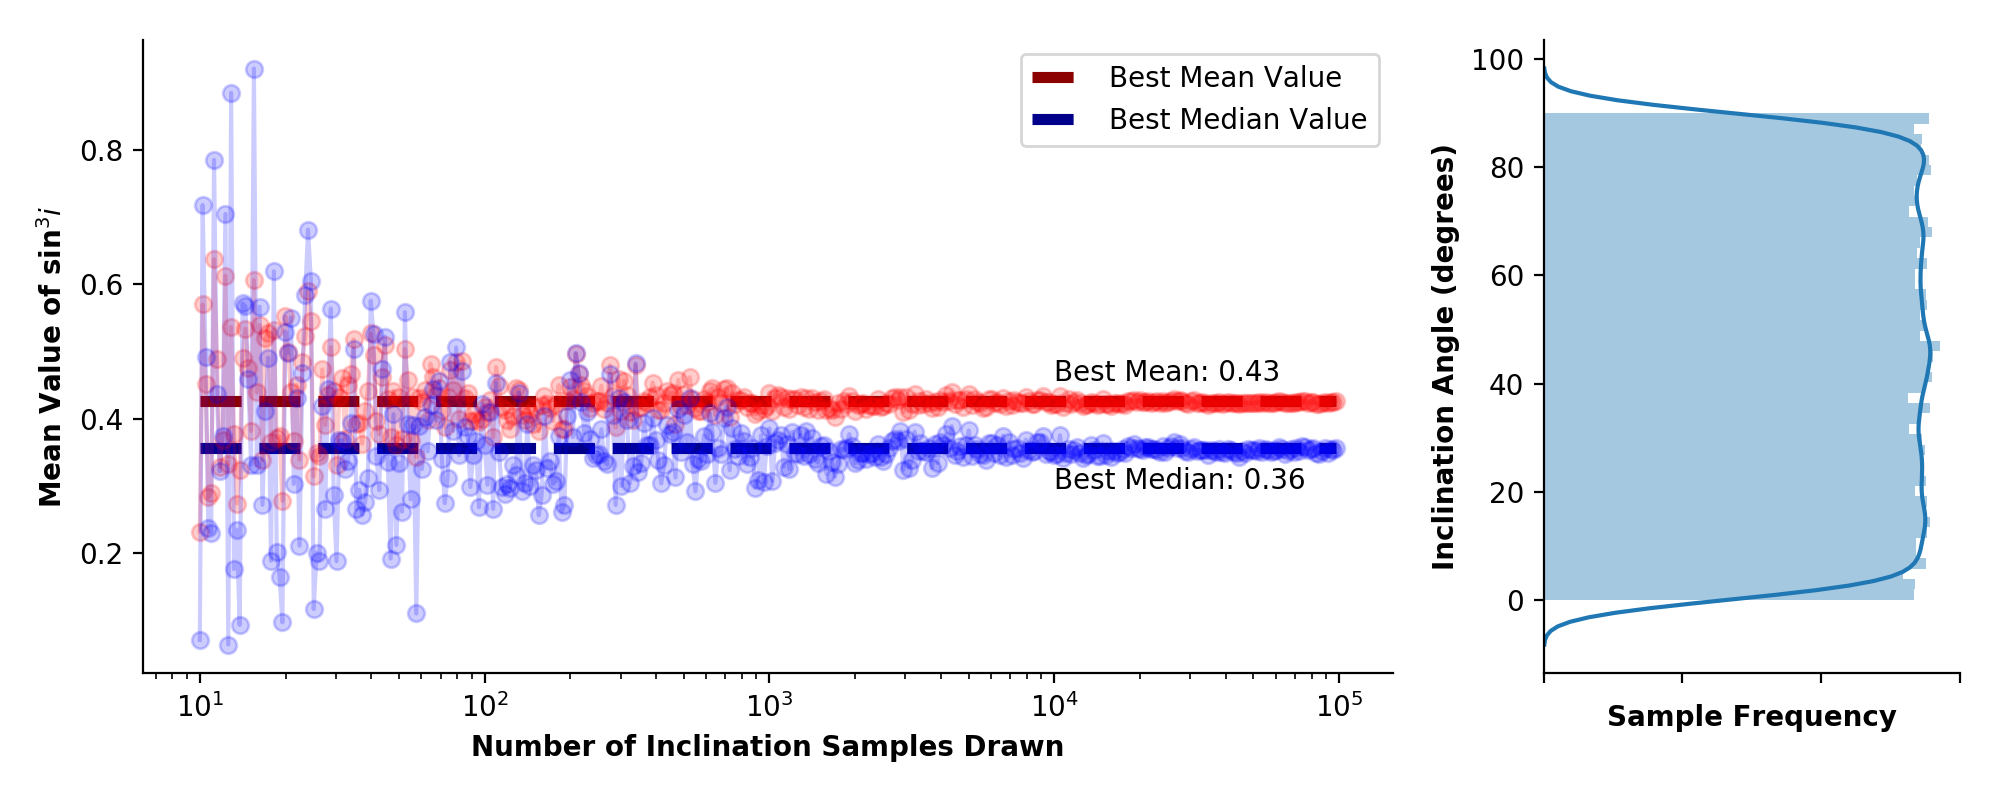
\includegraphics[width=\linewidth]{average_orbital_inclinations.png}\hfill%
  \hspace*{\fill}%
  \caption{The distribution of mean values of $\langle\sin^3 i\rangle$ over various sample sizes.}
  \label{fig:incls}
\end{figure}

Unfortunately, as shown in Fig. \ref{fig:incls}, this was not the case. The cause for the error in this plot is the characterization of the probability distribution. I chose a uniform distribution when writing this code (shown in the plot on the right - a flat, even sample of inclinations between 0 and 90$^o$), while it should be given by $\sin i$, which would push the mean higher and likely to 0.59, the expected value.

\end{answer}




\begin{problem}{6}
  Show that, if the surface of a pulsar were at the same temperature as the photosphere of the Sun, the pulsar would have M$_V \approx$ 30.
\end{problem}


\begin{answer}{6}
  We know that magnitude and luminosity are related by
  \begin{align*}
    M_1 - M_2 = -2.5 \log{\frac{L_1}{L_2}},
  \end{align*}

  where $M_1, M_2, L_1, and L_2$ are the absolute magnitudes and luminosities of sources $s_1$ and $s_2$, respectively. By letting $s_2$ be the Sun, we may substitude in its known magnitude and luminosity, find $L_1$, and thus solve for $M_1$.

  To do this, of course, we must solve for $L_1$. To do so, we may rearrange the effective temperature equation for luminosity, yielding $L = 4 \pi R^2 \sigma T^4$. Since we are told that the temperature of our source is the same as that of the Sun, we may thus rewrite our initial equation as
  \begin{align*}
    M_{\text{pulsar}} &= M_\odot -2.5 \log{\frac{4 \pi R_{\text{pulsar}}^2 \sigma T_{\odot}^4}{4 \pi R_{\odot}^2 \sigma T_{\odot}^4}} \\
        &= M_\odot -2.5 \log{\left[\left(\frac{R_\text{pulsar}}{R_{\odot}}\right)^2 \right]}
  \end{align*}

Looking up values, we find that pulsars - which are neutron stars - have masses of just $\sim$10 km, making the ration of radii become $\frac{R_\text{pulsar}}{R_{\odot}} = 10/(7 \times 10^5) = 1.43 \times 10^{-5}$. Another lookup indicates that the Sun's absolute magnitude is $M_\odot = 4.83$. Therefore,

\begin{align*}
  M_{\text{pulsar}} &= M_\odot -2.5 \log{\left[\left(\frac{R_\text{pulsar}}{R_{\odot}}\right)^2 \right]} \\
  &= 4.83 -2.5 \log{\left[\left(1.43 \times 10^{-5}\right)^2 \right]} \\
  &= 31.5
\end{align*}

This shows that, unsurprisingly, very small objects would be very faint if they didn't have giant spinning laser beams periodically flashing at us.
\end{answer}



%   % A TABLE
%   \centerline{\textbf{Results}}
%   \smallskip
%   \centerline{
%   \begin{tabular} {cc}
%   \hline \hline
%   l, b          & (324.52$^o$, 53.49$^o$) \\
%   M$_V$         & 6.19 \\
%   E(B-V)        & 0.75 \\
%   A$_V$         & 2.25 \\
%   d             & 30.48 pc \\
%   v$_{space}$   & 2628 km s$^{-1}$ \\
%   M$_{bol}$     & 5.9 \\
%   T$_e$         & 5040 \\
%   L/L$_\odot$   & 0.27 \\
%   M/M$_\odot$   & 0.72 \\
%   R/R$_\odot$   & 0.55 \\
%   \hline
%   \end{tabular}}
% \end{answer}
% \bigskip \bigskip



%\end{multicols*}
\vfill\eject
\clearpage


\lstinputlisting[language=Python]{scratch_hw3.py}



\end{document}
